\documentclass{beamer}%
\usepackage[T1]{fontenc}%
\usepackage[utf8]{inputenc}%
\usepackage{lmodern}%
\usepackage{textcomp}%
\usepackage{lastpage}%
\usepackage{graphicx}%
\usepackage{xcolor}%
\usepackage{tcolorbox}%
%
\title{Yair company}%
\author{Your Name}%
\date{\today}%
%
\begin{document}%
\normalsize%
\section{Company Name}%
\label{sec:CompanyName}%

         \begin{frame}{ Open-SQL Framework - Results}
    \begin{itemize}
        \item \textbf{Tested Models:}
        \begin{itemize}
            \item Llama2-7B and Code-Llama-7B
            \item Fine-tuned using proposed COT (SFTI-COT-SK-FULL)
            \item Zero-Shot learning
        \end{itemize}

   
        \item \textbf{Performance improvement:}
        \begin{itemize}
            \item \textbf{Llama2-7B}  from \(2.54\%\) to \(41.04\%\)
            \item \textbf{Code Llama-7B}  from \(14.54\%\) to \(48.24\%\)
        \end{itemize}
    \end{itemize}
\end{frame}
        

%
\section{Introduction}%
\label{sec:Introduction}%
\begin{frame}%
\frametitle{Introduction}%
This slide introduces the company and provides context.%
\end{frame}

%
\section{Data}%
\label{sec:Data}%
\begin{frame}%
\frametitle{Data}%
This slide contains the data used in the analysis.%
\begin{itemize}%
\item Hey%
\item $2^4 = ?$%
\end{itemize}%
\end{frame}

%
\section{Analysis}%
\label{sec:Analysis}%
\begin{frame}%
\frametitle{Analysis}%
This slide presents the analysis of the data.%
\end{frame}

%
\section{Classifications}%
\label{sec:Classifications}%
\begin{frame}%
\frametitle{Classifications}%
This slide presents the classifications based on the analysis.%
\end{frame}

%
\section{Financial Ratios}%
\label{sec:FinancialRatios}%
\begin{frame}%
\frametitle{Financial Ratios}%
This slide presents the calculated financial ratios:%
\begin{itemize}%
\item \textbf{Current Ratio}: 1.3471170068309741%
\item \textbf{Quick Ratio}: 0.5753283674088541%
\item \textbf{Immediate Liquidity Ratio}: 0.06551951008641155%
\item \textbf{Cashflow To Sales Ratio}: -0.5430760161596967%
\item \textbf{Net Profit Margin}: 0.11317365327045374%
\item \textbf{Operating Profit Margin}: 0.13308573851948943%
\item \textbf{Ebitda Ratio}: 0.2004729432785413%
\item \textbf{Roe}: 0.1334263006927202%
\item \textbf{Roa}: 0.0440440924673883%
\item \textbf{Leverage Ratio}: 0.18750811611831633%
\item \textbf{Equity To Assets Ratio}: 0.28071139140275814%
\item \textbf{Receivables Ratio}: 0.594029139396786%
\item \textbf{Customers Ratio}: 0.7948614960927065%
\item \textbf{Inventory Ratio}: 1.7950671937876375%
\item \textbf{Inventory Turnover Ratio}: 0.5570822103266088%
\item \textbf{Inventory Days}: 685.9749342669469%
\item \textbf{Payables Days}: 47.00758043484057%
\end{itemize}%
\end{frame}

%
\section{Visualizations}%
\label{sec:Visualizations}%
\begin{frame}%
\frametitle{Visualizations}%
This slide contains a simple line graph.%


\begin{figure}[h!]%
\centering%
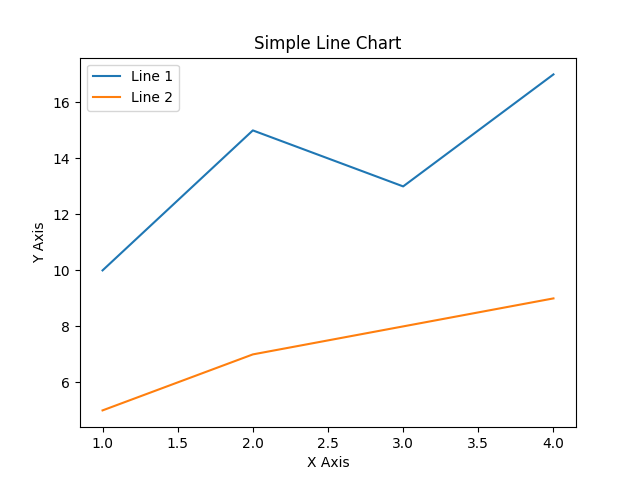
\includegraphics[width=80mm]{line_chart.png}%
\end{figure}

%
\end{frame}

%
\section{Anomalies}%
\label{sec:Anomalies}%
\begin{frame}%
\frametitle{Anomalies}%
This slide presents the detected anomalies in the data.%
\end{frame}

%
\section{Prediction}%
\label{sec:Prediction}%
\begin{frame}%
\frametitle{Prediction}%
This slide presents predictions based on the data.%
\end{frame}

%
\section{Conclusions}%
\label{sec:Conclusions}%
\begin{frame}%
\frametitle{Conclusions}%
This slide summarizes the key takeaways from the analysis.%
\end{frame}

%
\end{document}